Obtener el \textbf{estado, segmento} y el \textbf{total de clientes} que no han solicitado \textbf{ninguna orden}. \\

Dado esto, \textit{seleccionamos} todos los clientes de la relación \textit{customer}, almacenando dichas tuplas en una relación temporal \textit{clientes}. Luego, seleccionamos los IDs de los clientes que han realizado órdenes de la relación \textit{orders}, almacenando dichas tuplas en una relación temporal \textit{clientes\_con\_ordenes}. A continuación, obtenemos los IDs de los clientes que no han realizado ninguna orden mediante la operación de diferencia de conjuntos entre \textit{clientes} y \textit{clientes\_con\_ordenes}, almacenando el resultado en relación temporal \textit{clientes\_sin\_ordenes}. Finalmente, utilizamos el operador de proyección para obtener el \textbf{estado, segmento} y el \textbf{total de clientes} que no han solicitado \textbf{ninguna orden}. \\

La consulta en álgebra relacional se vería mas o menos de la siguiente manera: \\

\begin{center}
    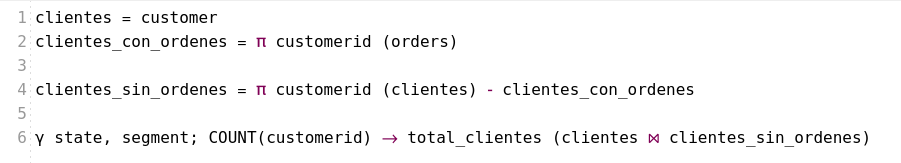
\includegraphics[width=14cm]{resources/pregunta2/2.5.1.png} \\
\end{center}

El árbol de la consulta: \\

\begin{center}
    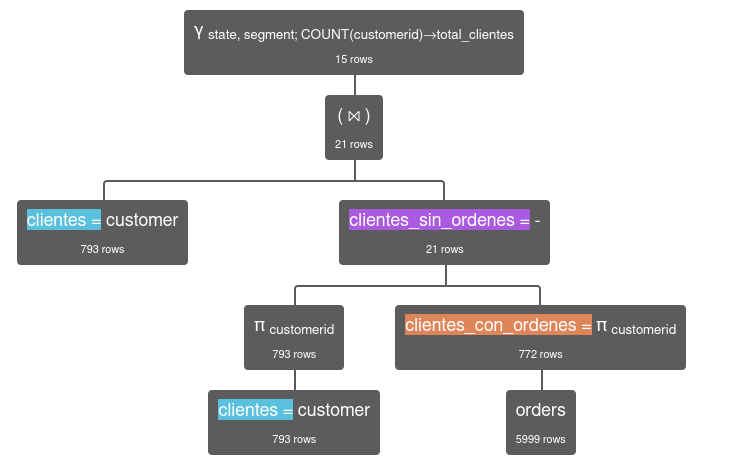
\includegraphics[width=14cm]{resources/pregunta2/2.5.2.png} \\
\end{center}

y la tabla resultante: \\

\begin{center}
    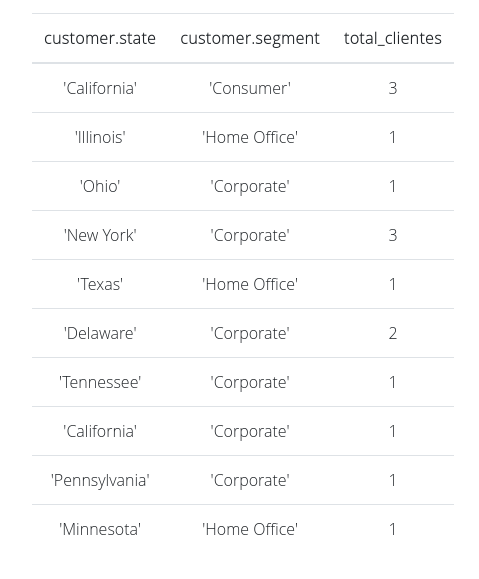
\includegraphics[width=10cm]{resources/pregunta2/2.5.3.png} \\
\end{center}
